\section{实验内容\cite{pcl2002}}

\subsection{仪器与药品}

\begin{figure}[H]
    \centering
    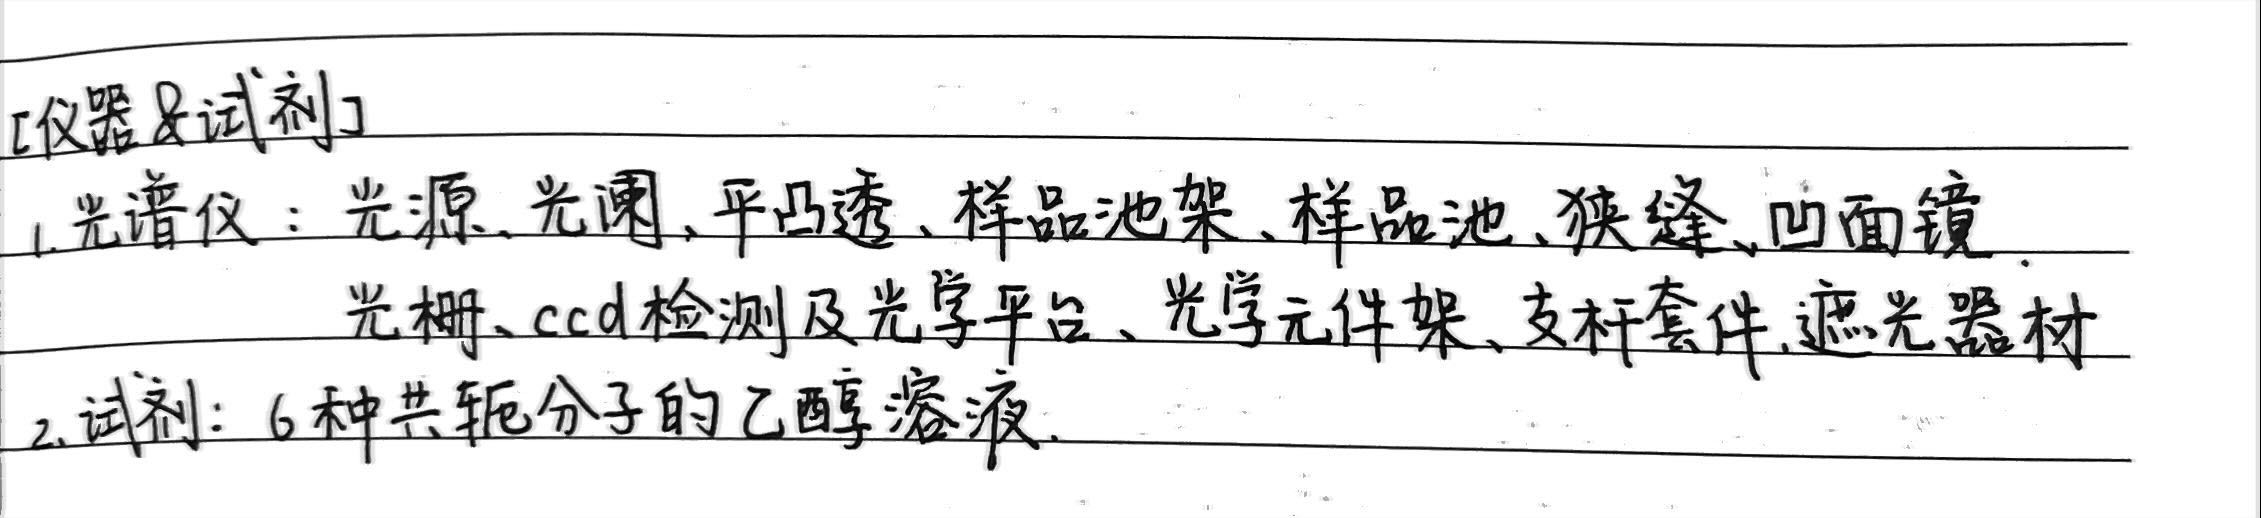
\includegraphics[width=.85\textwidth]{figures/0-2.jpg}
    \bicaption{预习报告:仪器与药品}{Preview report: instruments and reagents}
\end{figure}

\begin{table}[H]
    \centering
    \bicaption{6种共轭分子的代称、名称与结构}{Designations, names, and structures of six conjugated molecules}
    \begin{adjustwidth}{-2cm}{-2cm}
    \begin{center}
    \begin{tabular}{cccM{9cm}}
    \toprule
    代称 & 名称 & 浓度/\si{\mu mol\cdot L^{-1}} & 结构 \\
    \midrule
    \textbf{A1} & 3,3-二乙基硫菁碘盐 & 10 & 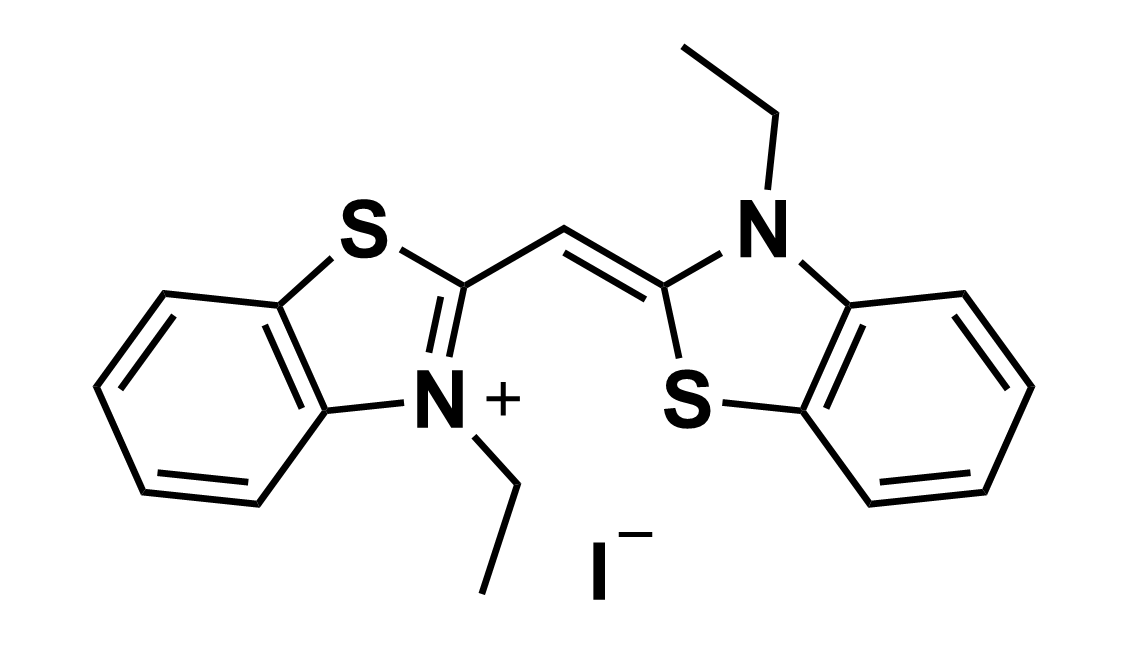
\includegraphics[scale=.18]{figures/0-A-1.png} \\
    \textbf{A2} & 3,3'二乙基嚷碳菁碘化物 & 5 & 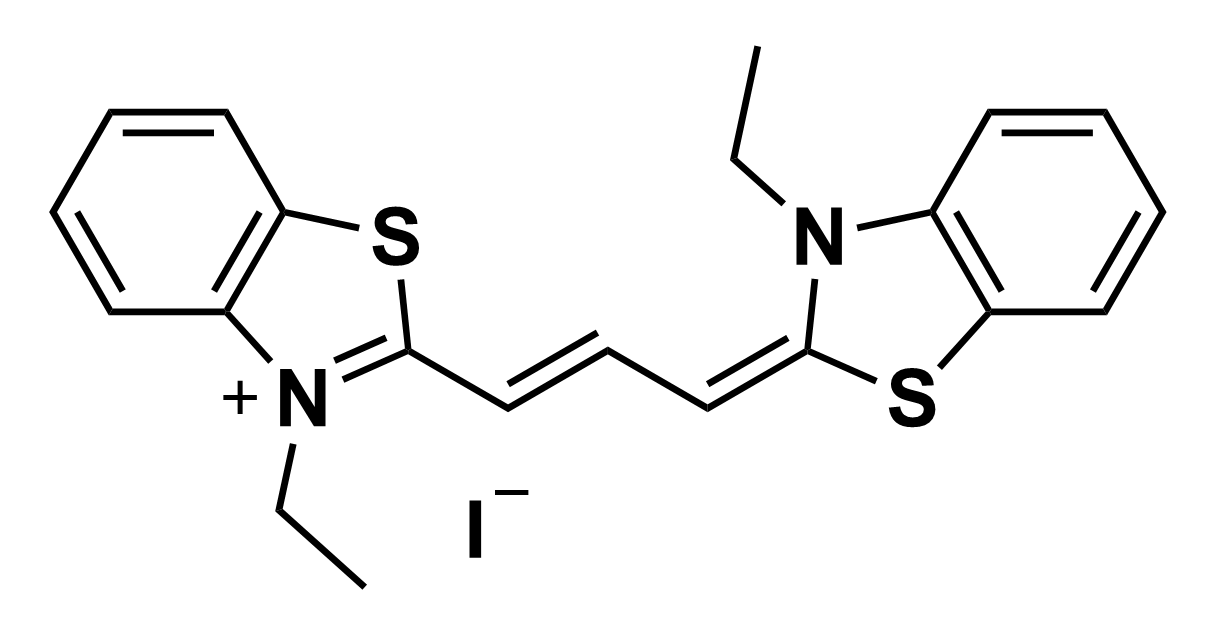
\includegraphics[scale=.19]{figures/0-A-2.png} \\
    \textbf{A3} & 3,3'-二乙基硫二炭花青碘 & 0.5,1,5,10,20,50& 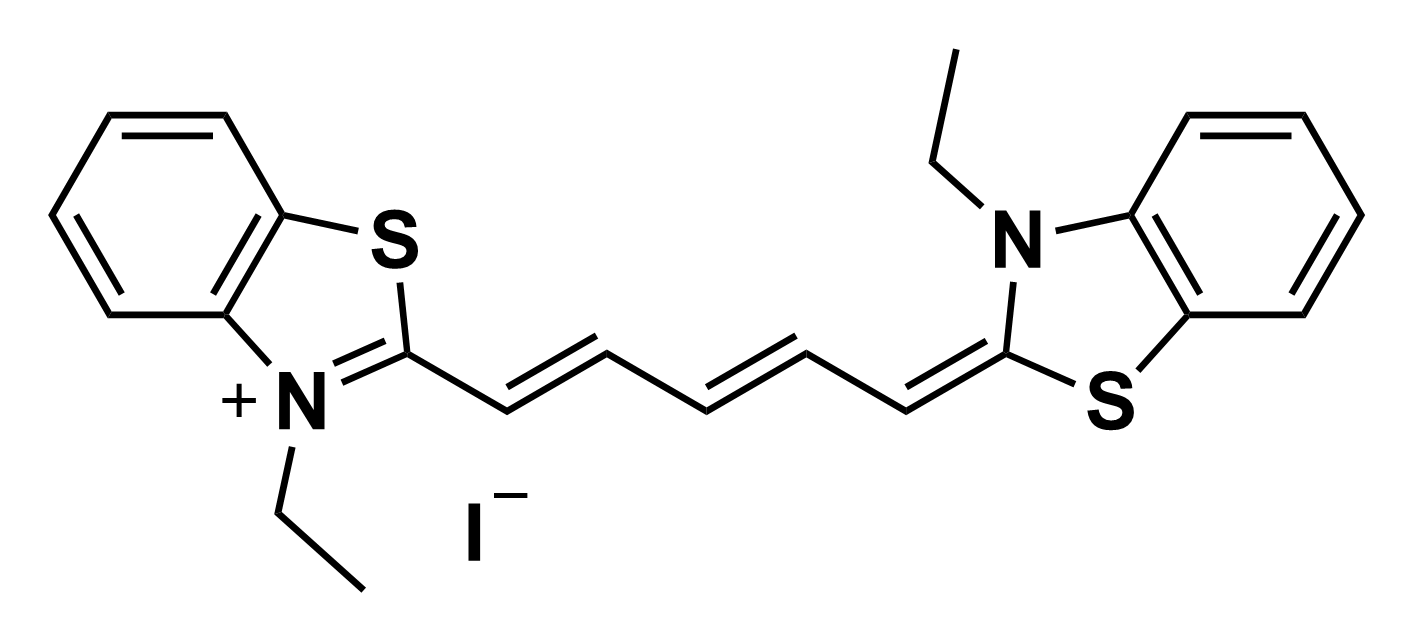
\includegraphics[scale=.2]{figures/0-A-3.png} \\
    \textbf{A4} & 3,3'-二乙基硫杂三羰花青碘化物 & 3 & 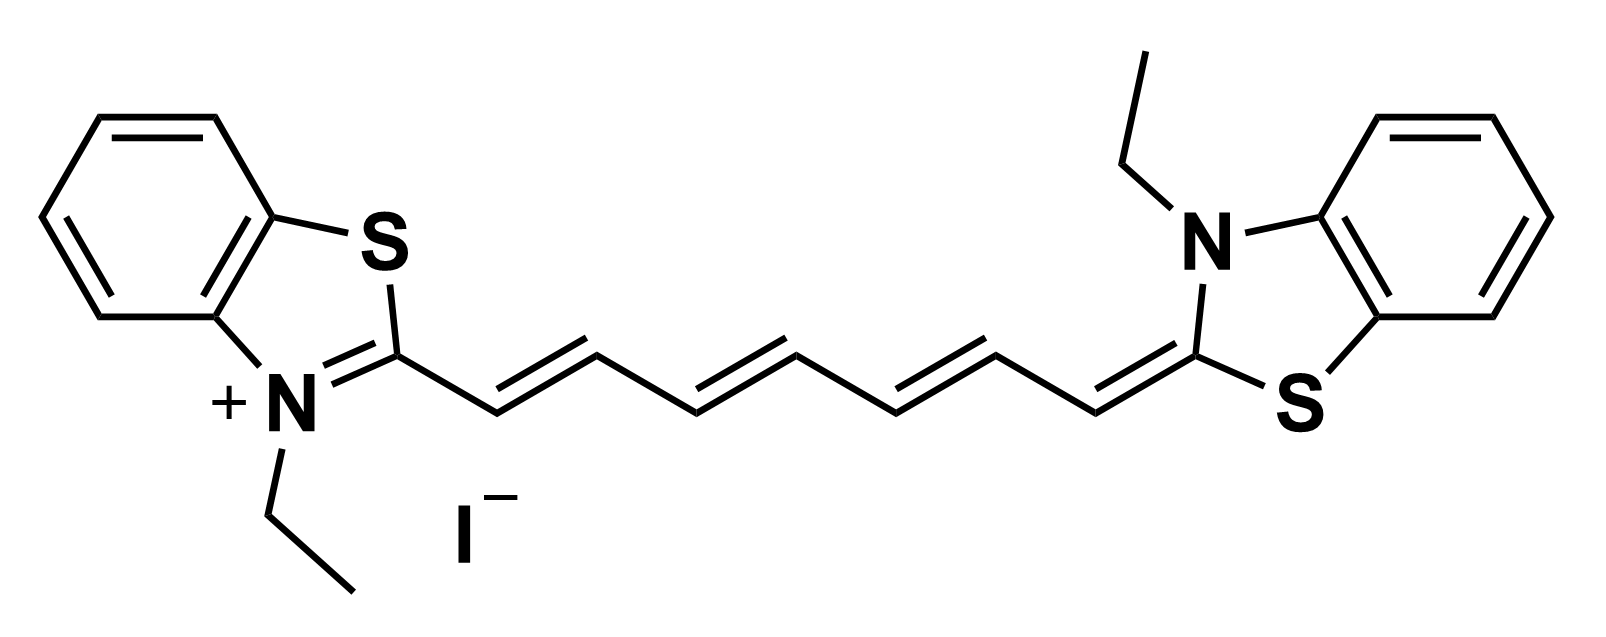
\includegraphics[scale=.2]{figures/0-A-4.png} \\
    \midrule
    \textbf{B1} & $\beta$-胡萝卜素 & 10 & 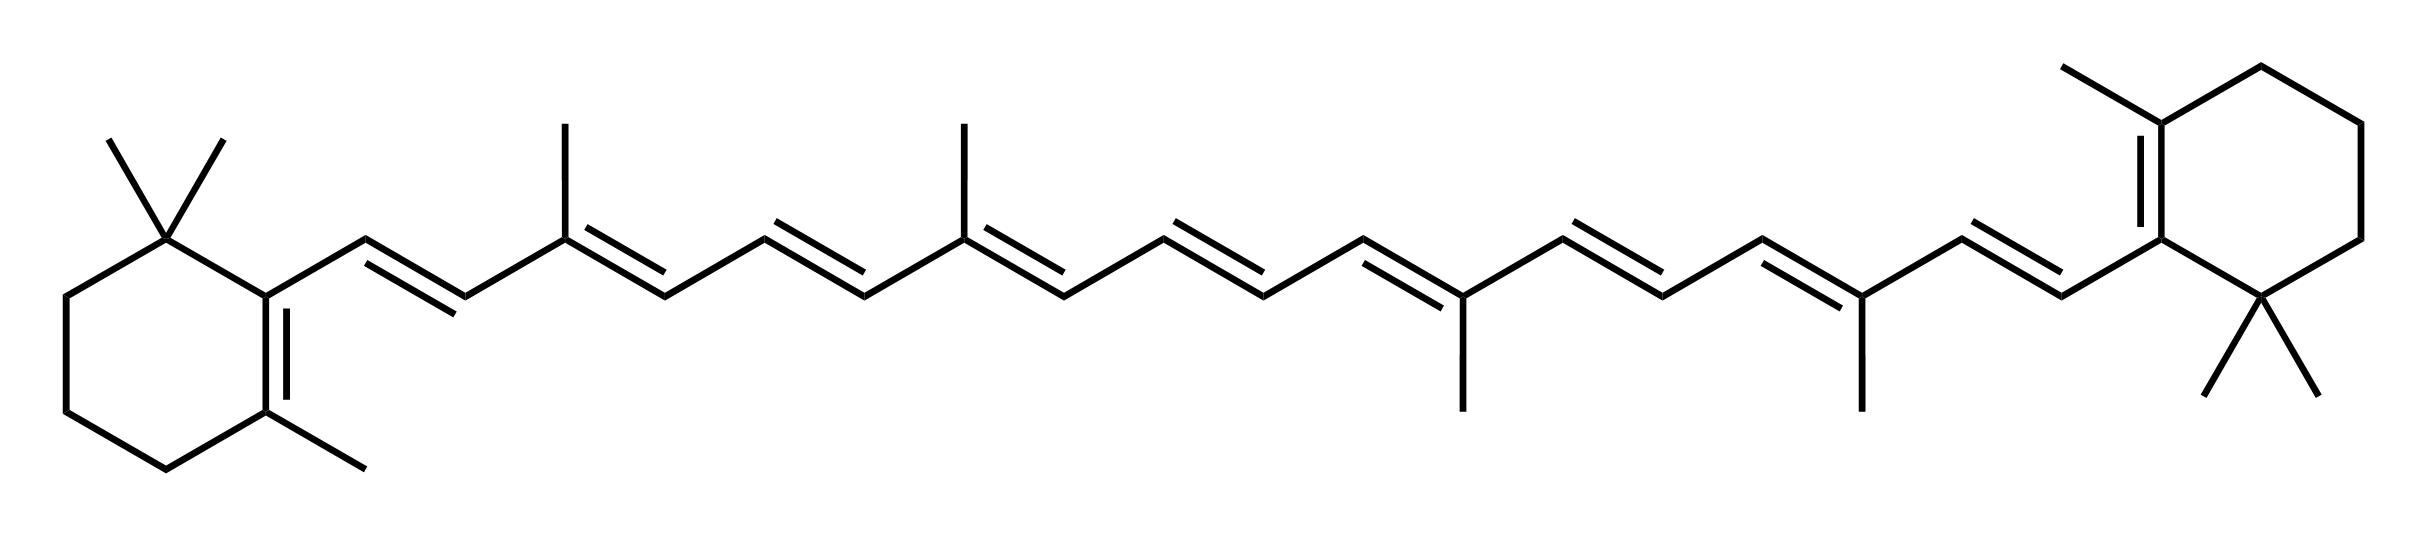
\includegraphics[scale=.2]{figures/0-B-1.png} \\
    \textbf{B2} & 2,6-二甲基-2,4,6-辛三烯 & 30 & 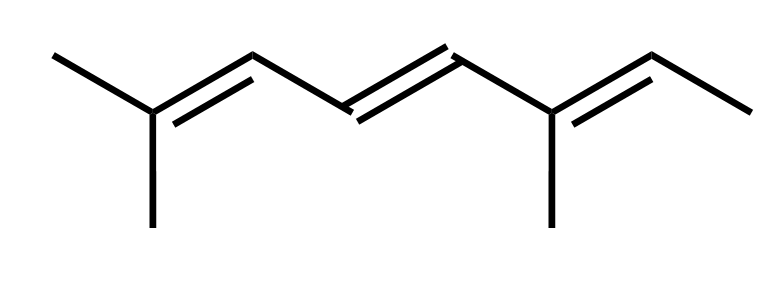
\includegraphics[scale=.2]{figures/0-B-2.png} \\
    \bottomrule
    \end{tabular}
    \end{center}
    \end{adjustwidth}
    \label{tab:0}
\end{table}

\subsection{实验步骤与条件}

\begin{figure}[H]
    \centering
    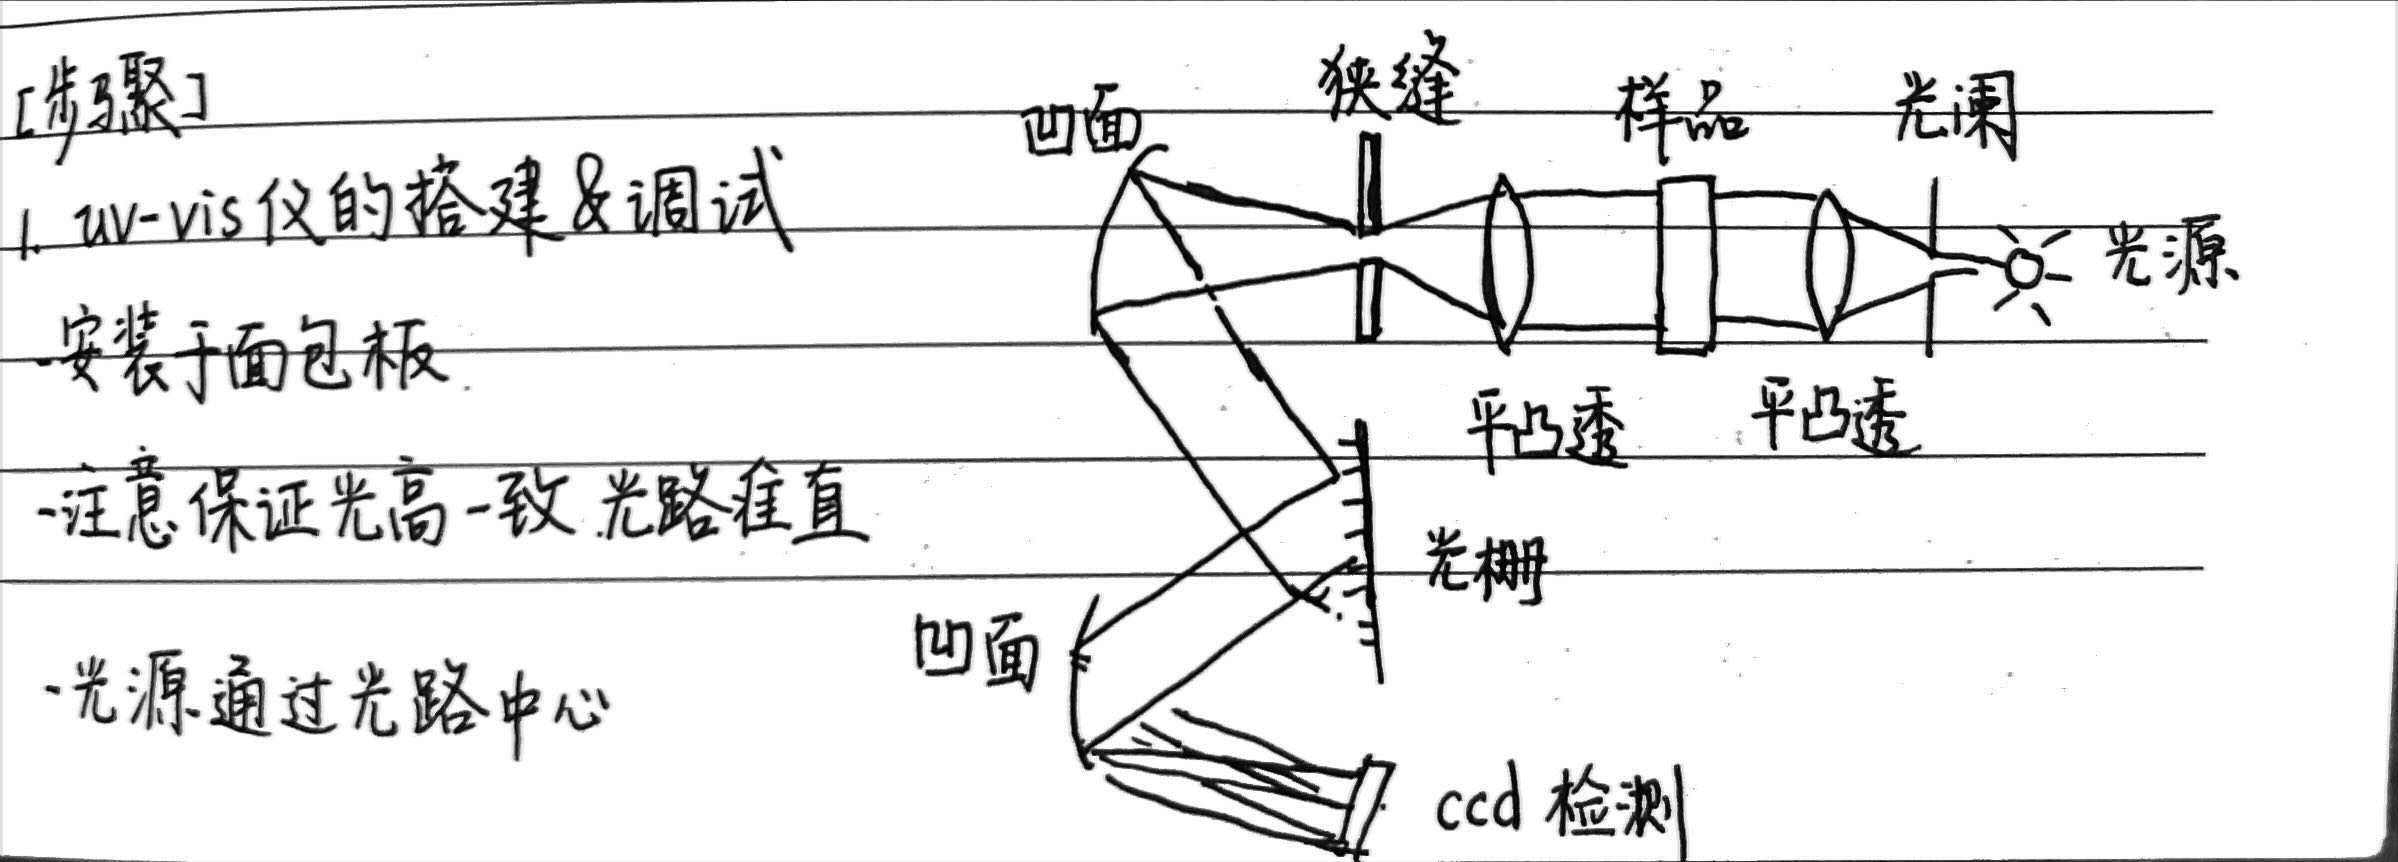
\includegraphics[width=.7\textwidth]{figures/0-3-1.jpg}
    \bicaption{预习报告:实验步骤与条件(1)}{Preview report: experimental procedures and conditions (1)}
\end{figure}

\begin{figure}[H]
    \centering
    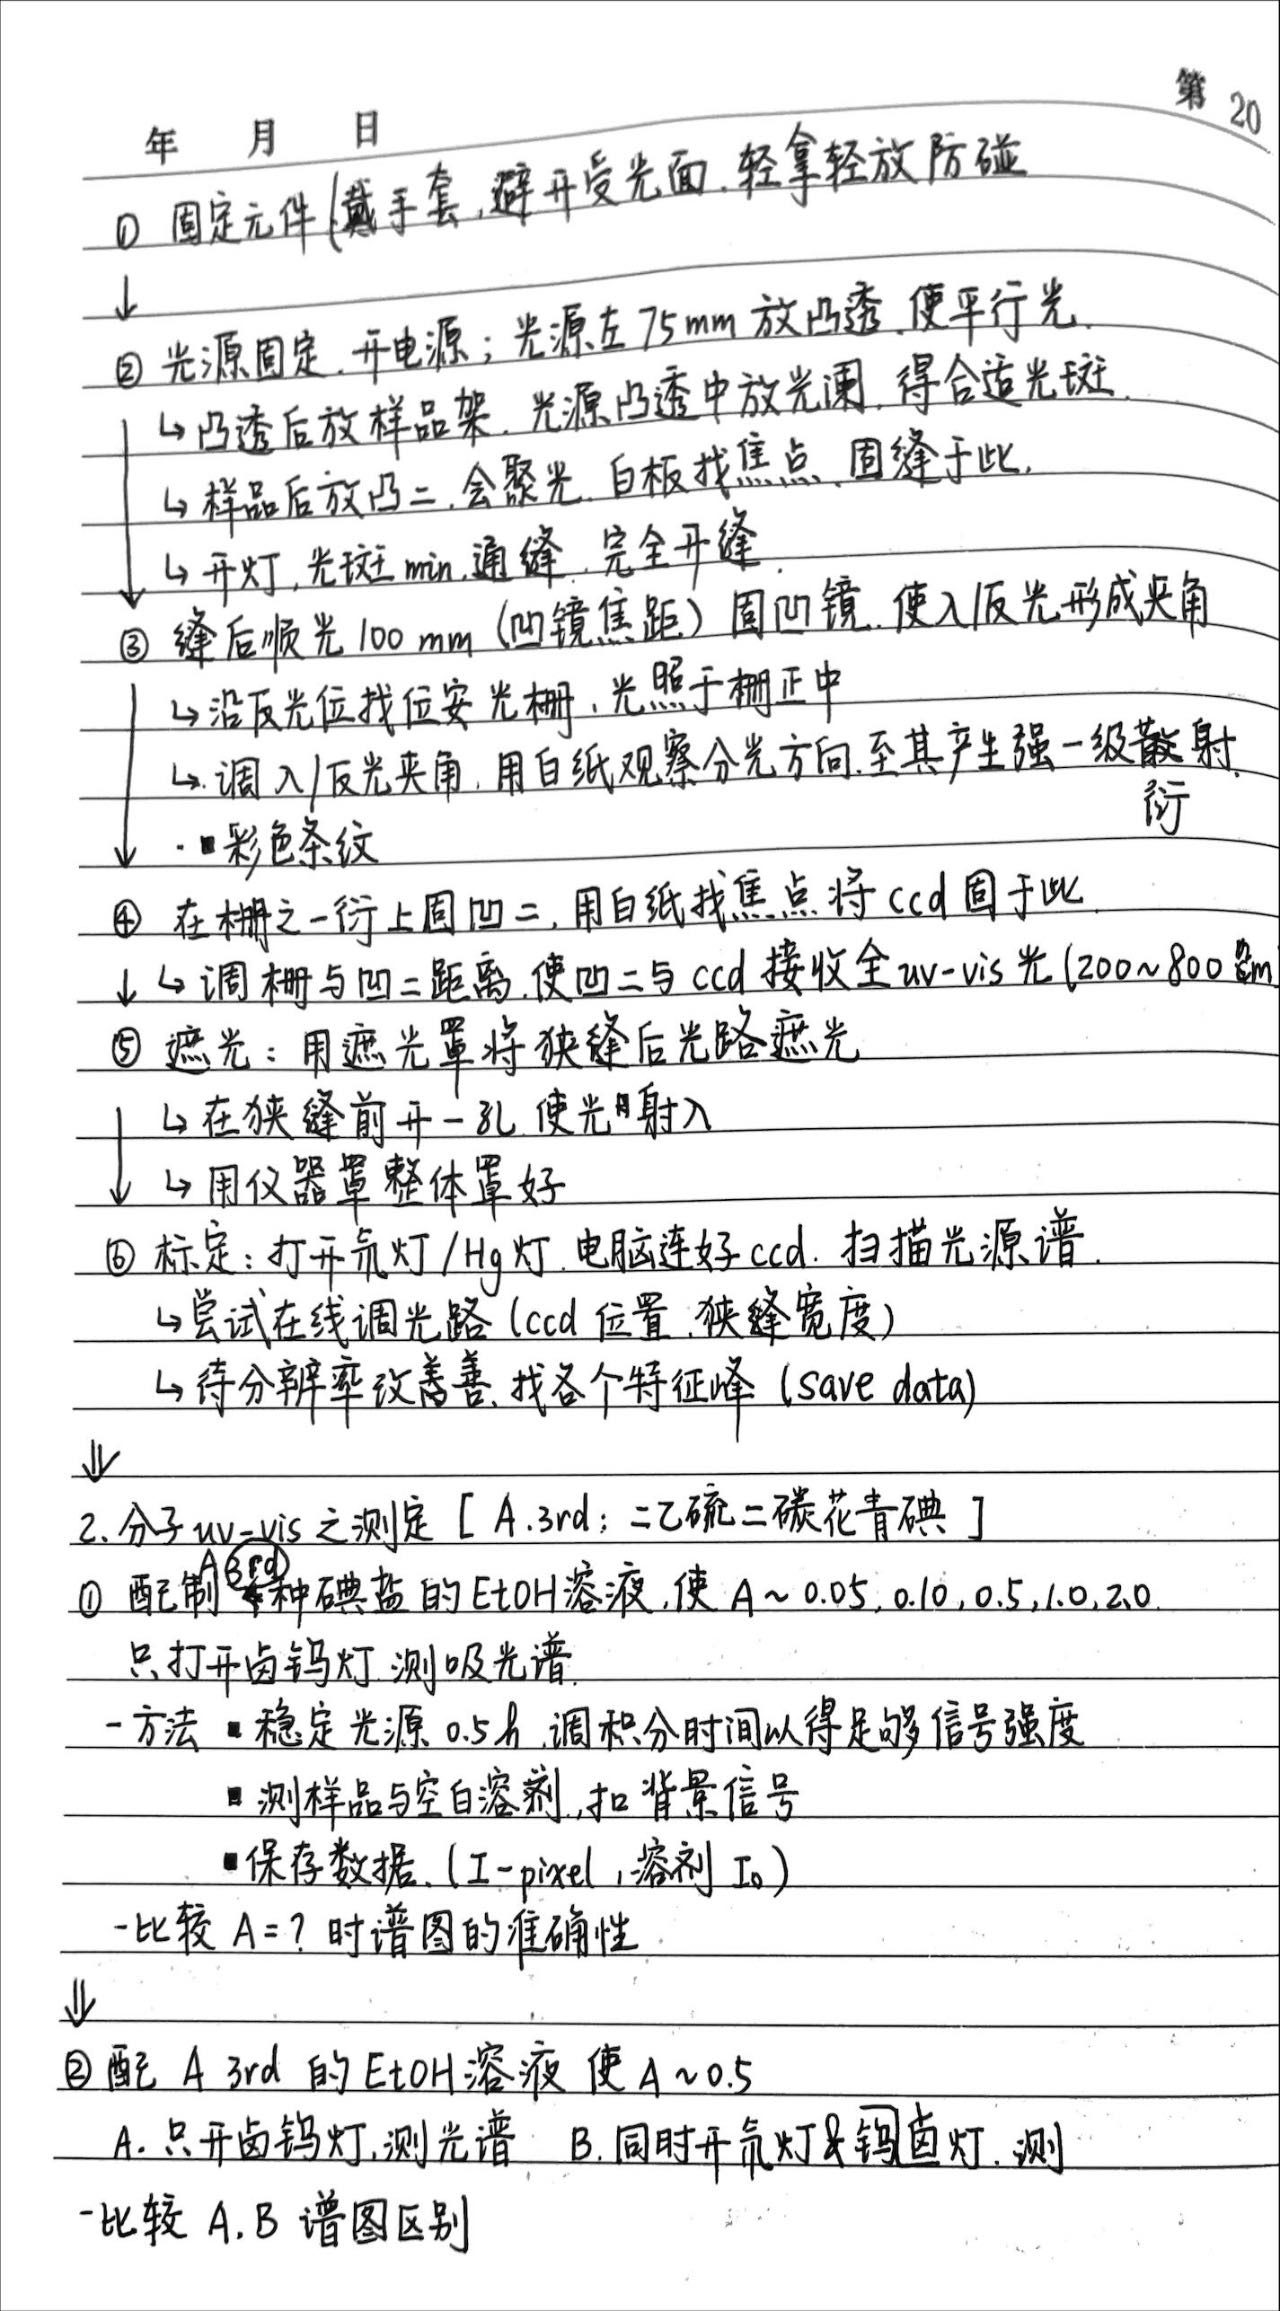
\includegraphics[width=.75\textwidth]{figures/0-3-5.jpg}
    \bicaption{预习报告:实验步骤与条件(2)}{Preview report: experimental procedures and conditions (2)}
\end{figure}

\begin{figure}[H]
    \centering
    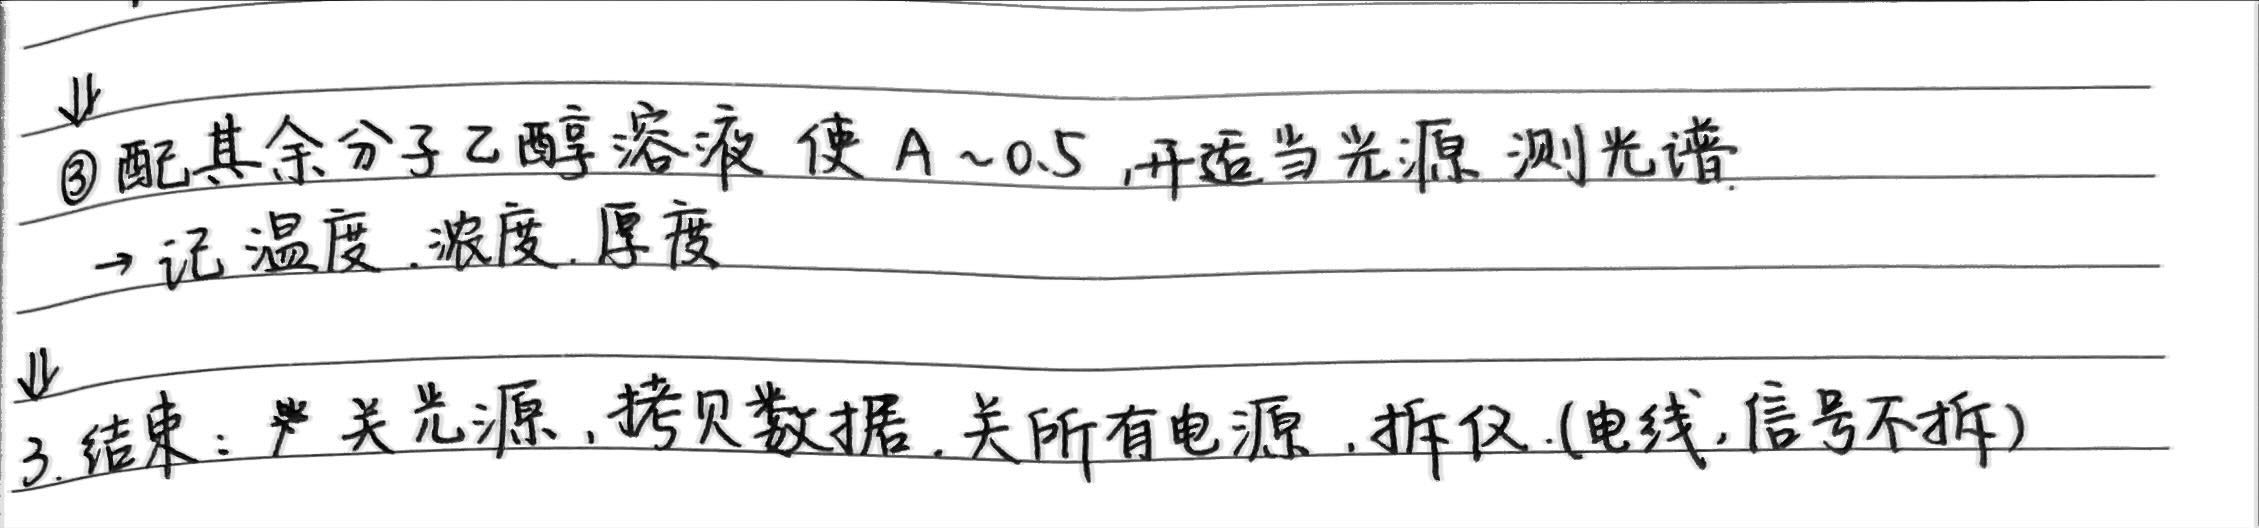
\includegraphics[width=.75\textwidth]{figures/0-3-4.jpg}
    \bicaption{预习报告:实验步骤与条件(3)}{Preview report: experimental procedures and conditions (3)}
\end{figure}

\subsubsection{紫外可见光谱仪的搭建}

将各个光学元件固定在元件架中,放回到光学支杆套杆上。打开氘灯电源,将凸透镜套组固定在光源左侧约 75\si{mm} 处,调整凸透镜高度,使透射光成为平行光;在凸透镜后适当位置固定样品池架,在光源和凸透镜之间安装光阑,使样品池获得合适的光斑;在样品池后适当位置安装第二个凸透镜套组,使光束形成会聚光,将可调狭缝固定于此处;打开卤钨灯,使得光斑最小且通过狭缝。

在狭缝后顺光方向约 100\si{mm} 处固定第一个凹面镜套组,使反射光与入射光成一尽量小的夹角,且反射光近似于平行光;沿反射光方向合适位置安装光栅套组,令光照在光栅的正中;反复调节光栅与入射光之间的夹角,用实验室提供的白纸板观察分光方向,直至得到较强的一级衍射。

在光栅的一级衍射方向上固定第二个凹面镜套组,用白纸板确定反射光焦点位置,将ccd 固定在此处;调整光栅与第二个凹面镜的距离。调节两次光谱仪,第一次,使凹面镜和 ccd 尽量接收到全部可见光以及近红外的光谱范围(400 $\sim$ 800\si{nm});第二次,使凹面镜和 ccd 尽量接收到紫外光与部分可见光的光谱范围(200 $\sim$ 700\si{nm})。

用实验室提供的纸板将狭缝及之后的光路仔细遮光,并在狭缝前的纸板上开一小孔,以便光线射入;再用纸板和遮光布将光谱仪罩好。

\subsubsection{光谱仪的标定}

打开氘灯光源,打开电脑,连接好 ccd,运行 ccd 控制软件,扫描光源谱图,在线调整光栅之后光路,对 ccd 的位置进行微调,观察分辨率的改善;观察到各特征峰足够明显时,彻底固定光栅之后光路和 ccd 的位置,找到氘灯各个特征峰。

对于可见-近红外光谱仪:利用氘灯 3 个特征峰对应的 ccd 像素值,作图拟合得到光谱仪的 $\lambda$−pixel 关系,对光谱仪进行标定。对于紫外-可见光谱仪:利用氘灯前 2 个特征峰对应的 ccd 像素值,解方程得到光谱仪的 $\lambda$−pixel 关系,对光谱仪进行标定。

\subsubsection{不同吸光度溶液、不同光源下的吸收光谱}

取不同浓度 A3 的乙醇溶液(浓度以此为0.5\si{\mu g\cdot L^{-1}}、1.0\si{\mu g\cdot L^{-1}}、5.0\si{\mu g\cdot L^{-1}}、10\si{\mu g\cdot L^{-1}}、20\si{\mu g\cdot L^{-1}}、50\si{\mu g\cdot L^{-1}}),以及A1、A2、A3、A4的乙醇溶液;只开卤钨灯,将卤钨灯光源稳定半小时,调整狭缝,调整积分时间为 20\si{ms};采集并扣除暗背景与空白溶剂的信号,保存各个样品的光谱数据并做图。

使用10\si{\mu g\cdot L^{-1}}的A3 乙醇溶液,同时打开卤钨灯和氘灯,调整狭缝,调整积分时间为 4\si{ms};采集并扣除暗背景与空白溶剂的信号,与只开卤素灯时的谱图进行作图对比,比较两种光源所得谱图的区别。

取A1、B1、B2的乙醇溶液,只开氘灯,将氘灯光源稳定半小时,调整狭缝,调整积分时间为 4\si{ms};采集并扣除暗背景与空白溶剂的信号,保存各个样品的光谱数据并做图。

\subsubsection{测定各共轭分子的吸收光谱} 

配制其他各共轭分子的乙醇溶液,打开适当光源,测定各分子的紫外可见吸收光谱,样品池厚度为 10 mm。
